\section{Introduction}
\label{intro}

When Internet traffic enters a country, it becomes subject to those
countries' laws.  As a result, users have more need than ever to
determine---and control---which countries their traffic is traversing.
An increasing number of countries have passed laws that facilitate mass
surveillance of their citizens~\cite{france_surveillance,
  netherlands_surveillance, kazak_surveillance, uk_bill}, and governments
and citizens are increasingly motivated to divert their Internet traffic
from countries that perform surveillance (notably, the United
States~\cite{russia_secure_internet,
  routing_errors, dte}).
% More recently, the Safe Harbor agreement,
%which allows the free flow of data between the US and the EU, 
%was struck down because it would give the NSA access to EU citizens'
%personal data~\cite{safe_harbour_illegal, safe_harbour_undecided}.  

Many countries---notably, Brazil---are taking impressive measures to reduce
the likelihood that Internet traffic transits the United
States~\cite{brazil_history, brazil_break_from_US, brazil_conference,
  brazil_conference2, brazil_human_rights} including building a 3,500
mile long fiber-optic cable from Fortaleza to Portugal (with no use of
American vendors); pressing companies such as Google, Facebook, and
Twitter (among others) to store data locally; and switching its dominant
email system (Microsoft Outlook) to a state-developed system called
Expresso~\cite{brazil_cable, brazil_us_companies}.  Brazil is also
building Internet Exchange Points (IXPs)~\cite{brazil_IXP1}, now has the
largest national ecosystem of public IXPs in
the world~\cite{brazil_ixp_ecosystem}, and the number of internationally
connected ASes continues to
grow~\cite{brazil_international_ases}. Brazil is not alone: IXPs are
proliferating in eastern Europe, Africa, and other regions, in part out
of a desire to ``keep local traffic local''. Building IXPs alone, of
course, cannot guarantee that Internet traffic for some service does not
enter or transit a particular country: Internet protocols have no notion
of national borders, and interdomain paths depend in large part on
existing interconnection business relationships (or lack thereof).  In
this paper, we present evidence to suggest that existing Internet
hosting and interdomain paths still make it difficult to avoid certain
countries for many popular websites. 

Prior work explored how central different countries are to interdomain 
routing based on simulated paths and an Internet topology~\cite{karlin2009nation}. 
Our study differs by actively measuring and analyzing the traffic originating in
five different countries: Brazil, Netherlands, Kenya, India, and the
United States.  Using RIPE Atlas probes and the MaxMind geolocation
service, we measure the country-level traffic paths for the Alexa Top
100 domains in each respective country.  Using the current state of
routing as a baseline for comparison, we then measure how avoidable a
given country is to a client in either Brazil, Netherlands, India,
Kenya, or the United States, using open resolvers and using an overlay
network.  Our contributions include: 

\begin{itemize}
\item The first in-depth measurement study of
  nation-state routing for Brazil, Netherlands, Kenya, India, and the
  United States. 
\item A preliminary evaluation of how open DNS resolvers and overlay
  network relays can help citizens and governments discover and use
  network paths that avoid certain countries.
\end{itemize}
\noindent
We find that hosting for many popular websites lacks diversity; in many
cases, even websites that are popular {\em locally} are hosted outside
the country where citizens are trying to access them. For example, more
than 50\% of the Alexa Top 100 domains in Brazil are hosted in the
United States. Internet paths also lack geographic diversity: About half
of the paths originating in Kenya to the most popular Kenyan websites
traverse the United States or Great Britain. Much of this phenomenon is
due to ``tromboning'', whereby an Internet path starts and ends in a
country, yet transits an intermediate country; for example, about 13\%
of the paths that we explored from RIPE Atlas nodes in Brazil to the
Alexa Top 100 in Brazil trombone through the United States. Fortunately,
our preliminary results suggest that the use of overlay network relays
to intentionally introduce network detours, and the use of open DNS
resolvers to discover hosting diversity can reduce tromboning and
generally help users select paths that avoid certain countries.

Our measurement study tackles two questions: (1)~Which countries do {\em
  default} Internet routing paths traverse?; (2)~What types of methods
can we use to take advantage of hosting and path diversity to help governments
and citizens better control transnational Internet paths?

Determining where a client's Internet traffic flows is complicated by
the complexity of websites~\cite{butkiewicz2011understanding}.  Many
websites embed content from other domains, which are most likely
hosted in different locations.  Therefore, the client has to make
additional web requests, which take different paths.  One initial web
request can result in content being fetched from many servers located
around the world, and to see where this traffic flows requires knowledge
of all paths from the client to requested sources (and all the requested
sources to the client).  Figure~\ref{fig:domains} shows the number of 
subsequent requests that are made from an initial web request for the 
Brazilian Alexa Top 100 domains.  Therefore, the first step of our measurement 
method is to {\tt curl} each of the Alexa Top 100 domains, and extract 
the third party domains from the response body.  Next, we use RIPE Atlas 
probes in the country of interest to locally resolve each domain and run 
traceroutes to the IP addresses in the DNS responses.  The measurements 
were run using Paris traceroute and each (probe, destination IP) pair 
was used twice: once using ICMP traceroute and once using TCP traceroute. 
Using MaxMind, each IP address was geolocated at a country granularity, 
and with the resulting set of country-level paths, we analyzed which 
countries host and/or transit the traffic.

\begin{figure}
\centering
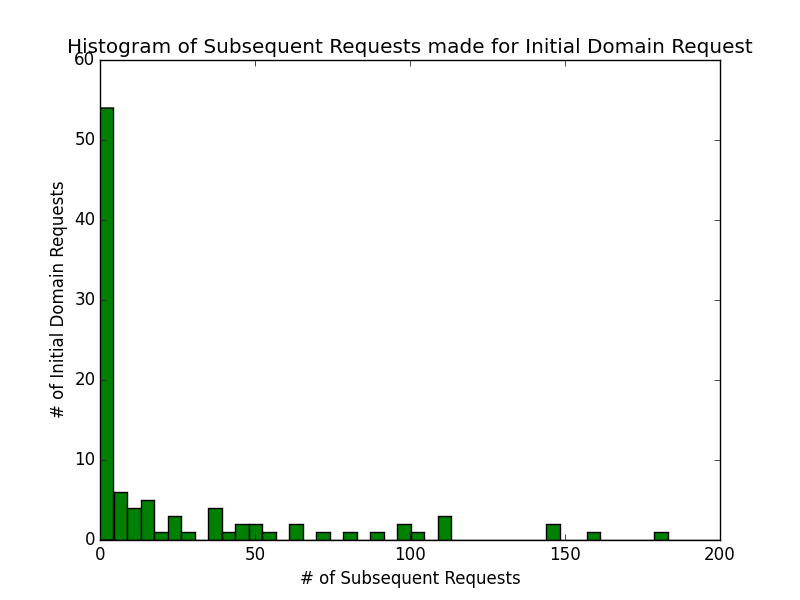
\includegraphics[width=.5\textwidth]{subsequent_request_hist}
\caption{A histogram of the number of third party requests are made by each initial domain request for the Brazilian Alexa Top 100 domains.}
\label{fig:domains}
\end{figure}

A client can use DNS open resolvers to discover georeplication of a site
or service that can facilitate the avoidance of specific countries. For
example, a client can query an open DNS resolver in a foreign country to
discover a different georeplicated instance of a service; this technique
(or the use of EDNS client subnet) can allow the client to discover
different replicas of the same service. The path to this newly
discovered replica may assist in avoiding particular countries
(particularly if the client is trying to avoid the country of the
original hosting replica!).  The increasing use of IP anycast can
sometimes make this technique
insufficient, however, if the client
receives the same IP address regardless of the apparent origin of the
DNS query.  Another approach is to use overlay network relays, which can
prevent the client from traversing an unfavorable country by introducing
a path that detours from the default. Additionally, using
relays in the client's country can somtimes help keep local traffic
local, by exploiting local paths that BGP does not select by default.
  
To evaluate the use of open resolvers as a tool for country avoidance, we
query open resolvers in geographically diverse locations around the world 
using the Alexa Top 100 domains.  Then we use RIPE Atlas probes to traceroute 
to the responses, and use MaxMind to generate country-level paths.  To evaluate 
overlay network relays for country-avoidance, we establish 12 relays in geographically 
diverse locations around the world, run traceroutes from the country of interest to 
each relay, as well as from each relay to the Alexa Top 100 domains.  After mapping 
the traceroutes to country-level paths with MaxMind, we measure which countries are 
avoidable.

After analysis, we present our main findings on hosting diversity, routing diversity, 
and avoidance feasibility.  

{\bf Hosting diversity.} We start by looking at hosting diversity, more specifically, how many
countries a domain is hosted in.  More diversity should provide for the
potential to avoid more countries.  About half of the
Alexa Top 100 domains in the five countries studied are hosted in more
than one country. 

{\bf Routing diversity.} Despite strong efforts made by some countries,
their traffic still traverses surveillance states, and is
subject to surveillance.  Over 50\% of the Alexa Top 100 domains in
Brazil and India are hosted in the United States, and over 50\% of the
paths from the Netherlands to the Alexa Top 100 domains transits the
United States.  About half of Kenyan traffic traverses the United States
and Great Britain.   

{\bf On the feasiblity of avoidance.} By measuring which domains are accessible without traversing a given
country using open resolvers and an overlay network, we see that
there are ways to circumvent unfavorable countries.  Without these
country avoidance techniques, Brazilian traffic transitted Spain, Italy,
France, Great Britain, Argentina, Ireland (among others), but using the
overlay network, Brazilian clients could completely avoid these
countries for the top 100 domains.  The overlay network can be used to
keep local traffic local; by using relays in the client's country, less
traffic trombones out of the client's country.  The percentage of paths
from the United States to the top 100 domains decreases from 11.2\% to 1.3\% when
relays are used.   

{\bf Cause for concern.} Unfortunately, some of the more prominent surveillance states are also
some of the {\textit least avoidable} countries.  Most countries are
highly dependent on the United States, a known surveillance state, and
not dependent on other countries.  Neither Brazil, India, Kenya, or the
Netherlands can completely avoid the United States with the country
avoidance techniques.  With the overlay network, both Brazilian and
Netherlands paths avoid the United States about 65\% of the time, and
the United States is completely unavoidable for about 10\% of the paths
because it is the only country where the content is hosted.  Kenyan traffic can
only avoid the United States on about 40\% of the paths from Kenya to
the top 100 domains.  On the other hand, the United States can avoid
every other country except for France and the Netherlands, and even then
they are avoidable for 99\% of the top 100 domains. 

This rest of this paper is organized as follows.  In the next section, we discuss
the current nation-states that conduct mass surveillance or are in the 
process of drafting laws for surveillance.  In
Section~\ref{datasets} we describe our measurement methods.
We point out the advantages and disadvantages of existing datasets, and
justify our decisions.  In Section \ref{measure}, we present results that show which countries
current Internet traffic is transiting and hosted in.  Next, Section
\ref{avoid_results} shows how well open DNS resolvers and relays work to avoid any
given country.  We discuss how our system differs from others and
uniquely suits the purpose of country avoidance in Section
\ref{discussion}, we review related work in Section \ref{related}, and
conclude in Section \ref{conclusion}. 
